\chapter{Software Implementation}
\lhead{\emph{Software Implementation}}

The following key technologies have been chosen for implementation of the Monitoring Application prototype.

\begin{itemize}
	
	\item \textbf{Java} version 8 (https://www.java.com) has been selected as the implementation language for prototype microservices, as the author has considerable experience with same.
	
	\item \textbf{Python} has been chosen as the implementation language for any command-line tooling developed as part of the prototype's supporting ecosystem.
		
	\item \textbf{Spring Boot} (https://spring.io/projects/spring-boot) is a popular, Java based application framework designed around the principle of convention-over-configuration \cite{Conventi95:online}. Spring Boot provides a powerful data access framework as well as out-of-the-box integration with popular messaging frameworks such as Kafka and RabbitMQ. Features such as integrated job scheduling and service discovery are key to the rapid development of several required application features. As an experienced Java developer, choice of this framework will minimise ramp-up time for the author. Spring Boot will underpin all microservices comprising this prototype.
	
	\item \textbf{Kafka} client for Java (https://kafka.apache.org). While the monitoring application prototype will be implemented in a technology-agnostic fashion in accordance with requirement  \textit{(NFR-2)}, plug-ins providing Kafka monitoring will be implemented using Kafka client libraries.
		
	\item \textbf{GraphQL} (https://graphql.org), developed by Facebook \cite{GraphQLA36:online}, has been chosen as the HTTP service interface implementation technology for all microservices providing same. An alternative to REST, GraphQL presents only a single client endpoint per service, supporting the query and mutation of service data. GraphQL servers present clients with schema metadata which allows for the development of powerful and intuitive client tools such as Insomnia IDE \cite{GraphQLI51:online}.
	
	\item \textbf{PostgreSQL} database (https://www.postgresql.org) has been chosen as the underlying persistence technology for the monitoring application. PostgreSQL's native support for persistence and querying of JSON data is a clear choice for persistence of monitored environment message payloads.
	
	\item The \textbf{WebSocket API} \cite{TheWebSo73:online}, part of the HTML5 specification, provides persistent full-duplex communication between centlient browsers and web servers. Asynchronous notifications will be pushed from Monitoring Application microservices to the Dashboard Client using this technology.
	
	\item \textbf{Dagre-d3} (https://github.com/dagrejs/dagre-d3) is a JavaScript library used to display directed graphs in web browsers. Based on the popular and powerful \textbf{D3} (https://d3js.org/) visualisation library,Dagre-d3 will underpin the Client Dashboard implementation.
	,
\end{itemize}

Additionally, \textbf{Kubernetes}, \textbf{Minikube},  \textbf{Kafka} and  \textbf{Zookeeper} will be extensively used in development of a test bed application, as described in Appendix A.

Implementation details for the various prototype microservices are explored in the following sections.

\section{Management Service}

This microservice is responsible for management and persistence of environment and topology state. An embedded web server hosting a GraphQL service provides a client interface for both users of the software and cooperating microservices, satisfying function requirement \textit{FR-6}. Users leverage the GraphQL interface to define and manage environment profile, environment, and topology information. Likewise, microservices such as the Aggregation and Discovery services communicate with the Management Service in order to enumerate monitored environment details and populate topography data. This microservice is implemented as a Spring Boot application, with a dependency on PostgreSQL database.

\subsection{Domain Model} \label{management_service_domain_model}
The domain model underpinning the Management Service has been designed with flexibility in mind. Environment configuration and topology models are sufficiently abstract to describe the properties of a pipeline application, without specific bindings to for example, Kafka related concepts. The data model underlying the Management Service is depicted in Figure \ref{mgmt_svc_domain_model}.

 \begin{figure}[H]
	\centering  
	\includegraphics[height=0.6\textheight]{figures/impl/mgmt/domain_package.png}
	\caption{Management Service data model.}
	\label{mgmt_svc_domain_model}
\end{figure}


The \textbf{Environment} model is the central type implemented by the Management Service. It models a single monitored environment, for example a Kafka-based pipeline application instance. An Environment comprises:
\begin{itemize}
	\item A unique name and UUID.
	\item A flag which indicates whether the environment is actively monitored.
	\item Exactly one associated \textbf{EnvironmentProfile}.
	\item Some number of associated \textbf{Configuration Properties}.
\end{itemize}

The \textbf{EnvironmentProfile} model specifies configuration information for a given class of environment, for example a Kafka or RabbitMQ-based application environment. Extending the Configurable model, the EnvironmentProfile specifies configuration properties which are read by various clients of the Management Service; the qualified class names of environment-specific monitoring task implementations are for instance provided as part of EnvironmentProfile. Additional attributes of the EnvironmentProfile are:
\begin{itemize}
	\item A unique profile identifier.
	\item An informational profile name.
\end{itemize}

An Environment may have at most one associated \textbf{Topology} instance. A Topology models a \textit{directed graph}, comprising one or more \textbf{Nodes}. A Node may have zero or more incoming and outgoing \textbf{Edges}. Every node has a name attribute, which is unique per topology. Every edge has a label attribute; multiple edges can share a common label.

A simplified example of the domain model for a given environment is given in Figure \ref{mgmt_svc_domain_model_example}. In this example, an EnvironmentProfile with profileId \textbf{KAFKA} has been defined. The profile defines a single configuration property named  \textbf{monitoringClass}. A single Environment is associated with this profile; the environment is named  \textbf{MyKafkaApp}, and is configured such that monitoring is enabled. A single configuration property, \textbf{bootstrap-server}, designates the host and port at which the environment's Kafka bootstrap server can be found. Finally, a simple topology comprising four nodes is associated with the environment.

 \begin{figure}[H]
	\centering  
	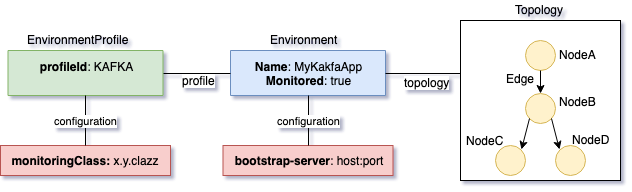
\includegraphics[width=\linewidth]{figures/impl/mgmt/mgmt_domain_example.png}
	\caption{Management Service simplified domain example.}
	\label{mgmt_svc_domain_model_example}
\end{figure}

\subsection{Modules}
The Management Service comprises the modules depicted in  \ref{mgmt_svc_modules}. The structure is typical of a Spring Boot based microservice.

\begin{figure}[H]
	\centering  
	\includegraphics[width=\linewidth]{figures/impl/mgmt/modules.png}
	\caption{Management Service modules.}
	\label{mgmt_svc_modules}
\end{figure}

\subsection{Component Interactions}
The Management Service presents a single external interface, detailed in the following sections. This interface provides various CRUD operations on Environments, EnvironmentProfiles, and Topology models. A GraphQL \textit {CommandResolver} implements the external interface. It in turn invokes a \texttt{ManagementService} interface, which further interacts with a JPA-based persistent model repository. The simple sequence diagram presented in Figure  \ref{mgmt_svc_seq_diagram} exemplifies the component interactions involved in enabling monitoring for a given environment.

 \begin{figure}[H]
	\centering  
	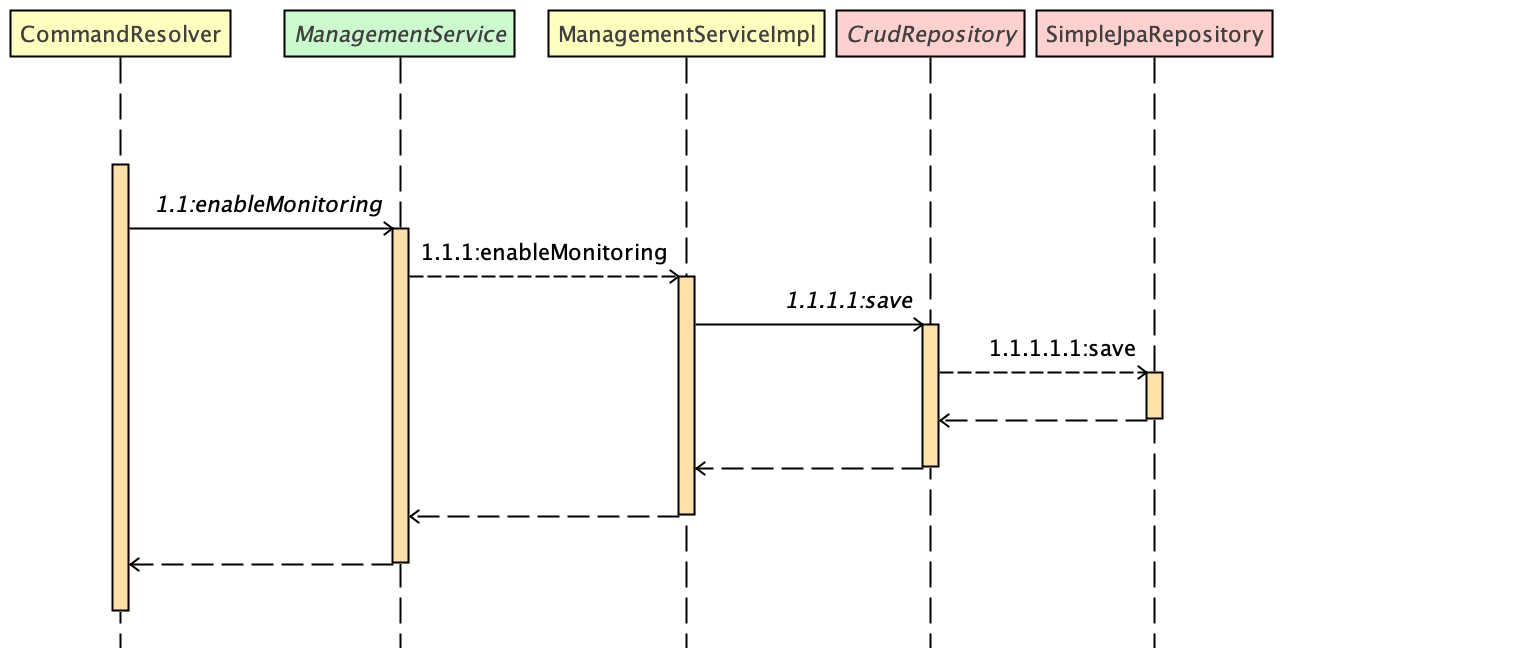
\includegraphics[width=\linewidth]{figures/impl/mgmt/enable_monitoring_seq.png}
	\caption{Sequence diagram: Enabling monitoring for an environment.}
	\label{mgmt_svc_seq_diagram}
\end{figure}

\subsection{External Interface} \label{management_service_external_interfaces}

The Management Service implements a GraphQL interface, providing CRUD operations across EnvironmentProfile, Environment, and Topology models. Both end users and other microservices are clients of this interface. End users are expected to interact directly with the GraphQL endpoint using suitable tooling. 

The Management Service implements a client module intended for import by other services; it abstracts the GraphQL interface, provided simple programmatic access to the service. Table \ref{mgmt_svc_graphql_operations} lists the various operations supported by the Management Service.

\vspace{10 mm}

\begin{table}[H]
	\centering
	\begin{tabular}{ |p{4cm}||p{4cm}| }
		\hline
		Domain Type& Operations \\
		\hline
		EnvironmentProfile   & register   \\
		& list   \\
		& delete   \\
		&     \\
		Environment &register \\
		&list \\
		&list monitored \\
		&update \\
		&delete \\
		&enable monitoring \\
		&disable monitoring \\
		&     \\
		Topology & register \\
		& list \\
		& update \\
		& delete \\
		\hline
		\end{tabular}
	\caption{Management Service GraphQL operations.}
		\label{mgmt_svc_graphql_operations}
\end{table}

\newpage
 
\section{Monitoring Service}

This microservice is responsible for the persistence of message traffic observed in monitored environments. It depends upon the Management Service for discovery of monitored environment information, synchronising periodically in order to start and stop concurrently executing environment monitoring tasks, partially satisfying functional requirement \textit{FR-5}. The implementation is agnostic of messaging technologies, in accordance with non-functional requirement \textit{NFR-2}. A \textit{MonitoringTask API} provides for the addition of technology-specific monitoring task implementations to this service, satisfying non-functional requirement \textit{NFR-1}; a Kafka-specific implementation has been provided with this prototype. Monitored environment messages are persisted, with a configurable retention period set by default to one hour. Furthermore, the module exports a data access module which is used by co-operating microservices such as the Aggregation Service. This microservice is implemented as a Spring Boot application, with a dependency on PostgreSQL database.

\subsection{Domain Model}
The Monitoring Service implements a simple domain model, comprising a single type \textbf{Message}. A Message represents a single message observed in a monitored environment. It comprises:

\begin{itemize}
	\item The identifier of the environment in which the message was observed.
	\item The edge label. While the Message type is technology agnostic, for a message observed in a Kafka-based environment, this attribute will correspond to a Kafka topic name.
	\item The source node name. In a Kafka-based environment, this attribute designates the message producer.
	\item The message content.
	\item The message timestamp.
\end{itemize}

The data model is depicted in Figure \ref{monitoring_svc_domain_model}.

\vspace{10 mm}

 \begin{figure}[H]
	\centering  
	\includegraphics[scale=1.8] {figures/impl/monitor/domain_package.png}
	\caption{Monitoring Service domain model.}
	\label{monitoring_svc_domain_model}
\end{figure}

\subsection{Modules} \label{monitoring_service_modules}
The Monitoring Service comprises the modules depicted in  \ref{monitoring_svc_modules}. The structure is typical of a Spring Boot based microservice.

\begin{figure}[H]
	\centering  
	\includegraphics[width=\linewidth]{figures/impl/monitor/modules.png}
	\caption{Monitoring Service modules.}
	\label{monitoring_svc_modules}
\end{figure}

\subsection{Component Interactions} \label{monitoring_service_interactions}

The Monitoring Service does not implement any external interfaces. It is driven by a scheduled synchronisation task which executes at a configurable interval, by default every five seconds. The synchronisation task first determines the set of currently monitored environments by polling the Management Service via its client module, as described in section \ref{management_service_external_interfaces}. The component interactions are depicted in Figure \ref{monitoring_sync_task_sequence}.

\begin{figure}[H]
	\centering  
	\includegraphics[width=\linewidth]{figures/impl/monitor/sync_task_seq.png}
	\caption{Monitored Environment synchronisation.}
	\label{monitoring_sync_task_sequence}
\end{figure}

The synchronization task now passes the set of monitored environment definitions to the \texttt{MonitoringService} interface; the implementation creates new monitoring tasks for environments which are not already subject to monitoring, while stopping any redundant monitoring tasks.

A \texttt{MonitoringTask} instance models a single environment monitoring job; an instance of MonitoringTaskFactory in module \textit{monitoring-service-job} dynamically instantiates such tasks via inspection of the \texttt{EnvironmentProfile} associated with a given \texttt{Environment} instance (see section \ref{management_service_domain_model}).

A single concrete implementation of the  \texttt{MonitoringTask} interface has been implemented. This task  implements the functionality required to perform monitoring a Kafka environment. It performs the following  steps in a dedicated monitoring thread:

\begin{itemize}
	\item Determine all known topic names via the Kafka client API.
	\item Create a dedicated monitoring thread.
	\item Create a Kafka consumer for the configured environment, configured to poll indefinitely.
	\item For each incoming Kafka message:
	\begin{itemize}
		\item Create a new \textit{Message} domain object.
		\item Set the message edge label to the name of the topic on which the message was received.
		\item Determine the message source node name via header inspection. The approach used to achieve header injection is described in section \ref{kafka_producer_header_design}.
		\item Set the message content to that of the received Kafka message.
		\item Set the Message timestamp and environment UUID.
		\item Save the message to a persistent JPA repository.
	\end{itemize}
\end{itemize}

\subsection{Monitoring Task API}
To extend the functionality of the software via addition of additional monitoring tasks for various technologies , the \texttt{MonitoringTask} interface must be implemented, and the implementation class(es) made available on the runtime classpath of the Monitoring Service. The service will dynamically instantiate such task implementations based on environment profile configuration as described in section \ref{monitoring_service_interactions}. This simple API provides methods for initialisation of the task with environment information and a \texttt{MessageRepository} instance. Additional methods instruct the monitoring task to start/stop execution.

\begin{figure}[H]
	\centering  
	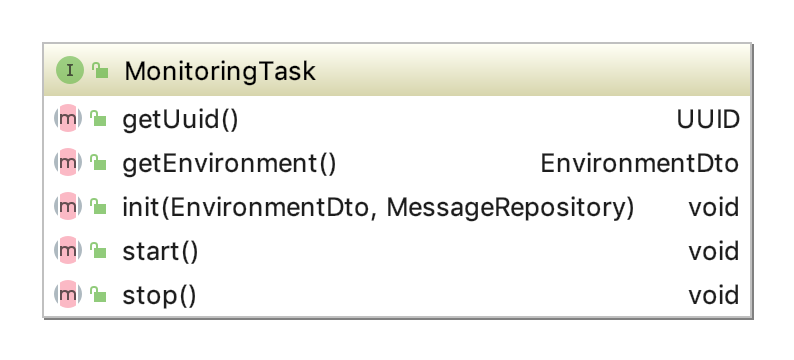
\includegraphics[scale=2.0]{figures/impl/monitor/monitoring_task.png}
	\caption{MonitoringTask API.}
	\label{monitoring_task_api}
\end{figure}


\subsection{Message Repository} \label{monitoring_service_message_repository}
The Monitoring Service defines a DAO module which is used by other microservices (specifically, the Aggregation Service and the Message Correlation Discovery Agent as discussed later in this document) to perform message lookup. This functionality is provided by an implementation of]  a \texttt{MessageRepository} interface, which defines methods for finding all environment messages in a given temporal window, finding the first and last messages for a given environment, finding the next sequential message for a given environment and edge and so on. A generic \texttt{executeQuery} method is provided for clients with esoteric query requirements. The interface class diagram is given in Figure \ref{monitoring_sync_message_repository}.

\begin{figure}[H]
	\centering  
	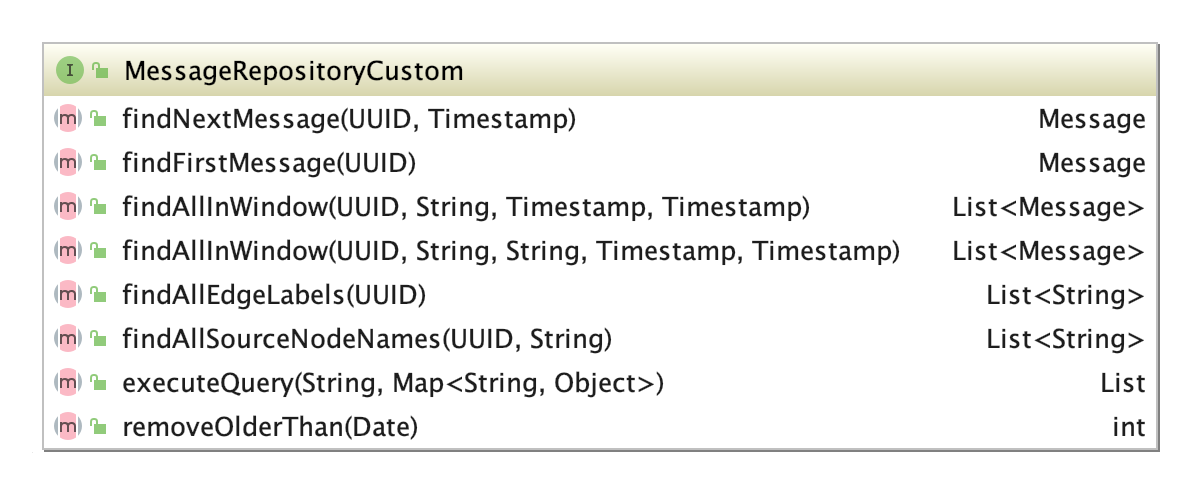
\includegraphics[width=\linewidth]{figures/impl/monitor/message_repository.png}
	\caption{Monitoring Service MessageRepository interface.}
	\label{monitoring_sync_message_repository}
\end{figure}

\subsection{Message Retention} \label{monitoring_service_message_retention}
The \texttt{Purge} module depicted in section \ref{monitoring_service_modules} is responsible for the flushing of persisted messages; the purge operation is performed at a configurable interval, with messages older than a configurable retention period being deleted from persistent storage. This functionality is intended to limit the application's use of disk space. 
\newpage

\section{Aggregation Service}

This microservice is responsible for the aggregation of message traffic persisted by the Monitoring Service, satisfying functional requirement \textit{FR-2}. Furthermore, it is responsible for the near real-time dispatch of aggregation data to interested parties such as the Dashboard Client. Environment aggregations for multiple monitored environments are performed in parallel for a one-second rolling window, implementing functional requirement \textit{FR-5}. Aggregations are persisted, with a configurable retention period set by default to one hour. Asynchronous aggregation notification are pushed to clients using Spring WebSocket support. This microservice is implemented as a Spring Boot application, with a dependency on PostgreSQL database. It leverages a data access module exported by the Monitoring Service for lookup of persisted messages.


\subsection{Domain Model} \label{aggregation_service_domain_model}
The Aggregation Service domain model comprises two models.The first, \texttt{EvironmentAggregation}, models aggregations across all edges for a given environment and temporal window. Every \texttt{EvironmentAggregation} has zero or more associated  \texttt{EdgeAggregation}s, which in turn model the number of messages observed for a given edge label and source node name.

 \begin{figure}[H]
	\centering  
	\includegraphics[scale=3.0] {figures/impl/aggregation/domain_package.png}
	\caption{Aggregation Service domain model.}
	\label{aggregation_svc_domain_model}
\end{figure}

An example of this domain model is given in Figure \ref{aggregation_svc_domain_model_example}. In this example, a single environment aggregation has been performed for a one-second window ending at time 18:09:51. The environment aggregation comprises aggregations for edges \textit{source}, \textit{validated} and \textit{ingest}. 5 messages have been aggregated on each of these edges during the one-second aggregation window.

\begin{figure}[H]
	\centering  
	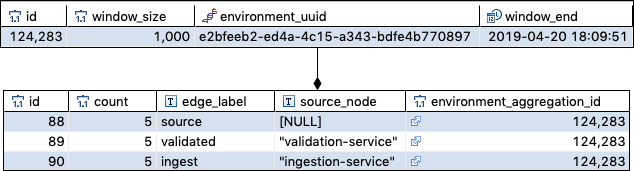
\includegraphics[width=\linewidth]{figures/impl/aggregation/domain_example.png}
	\caption{Aggregation Service domain example.}
	\label{aggregation_svc_domain_model_example}
\end{figure}

\subsection{Modules}\label{aggregation_service_modules}
The Aggregation Service comprises the modules depicted in  \ref{aggregation_svc_modules}. The structure is typical of a Spring Boot based microservice.

\begin{figure}[H]
	\centering  
	\includegraphics[width=\linewidth]{figures/impl/aggregation/modules.png}
	\caption{Aggregation Service modules.}
	\label{aggregation_svc_modules}
\end{figure}

\subsection{Component Interactions}

The Aggregation Service is driven by a scheduled synchronisation task which executes at a configurable interval, by default every five seconds. The synchronisation task first determines the set of currently monitored environments by polling the Management Service via its client module, as described in section \ref{management_service_external_interfaces}. The component interactions are depicted in Figure \ref{aggregation_sync_task_sequence}.

\begin{figure}[H]
	\centering  
	\includegraphics[width=\linewidth]{figures/impl/aggregation/sync_task_seq.png}
	\caption{Monitored Environment synchronisation.}
	\label{aggregation_sync_task_sequence}
\end{figure}

The synchronization task now passes the set of monitored environment definitions to the \texttt{AggregationService} interface; the implementation creates new aggregation tasks for environments which are not already subject to aggregation, while stopping any redundant aggregation tasks.

An \texttt{AggregationTask} instance models a single environment aggregation job; an instance of AggregationTaskFactory in module \textit{aggregation-service-job} is responsible for task instantiation. Each aggregation tasks leverages a MonitoringRepository instance (see Section \ref{monitoring_service_message_repository}) to collate recently monitored messages, aggregating message counts across a configurable aggregation window, which is sized to one second by default.

Each aggregation tasks runs in a dedicated thread, executing on condition that the aggregated environment is configured for monitoring at the Management Service. Aggregation tasks perform an initial check for unaggregated historical messages at task startup; if such messages are discovered, historical aggregation is performed. 

Whenever a new \texttt{EvironmentAggregation} is created, a notification is dispatched to any \texttt{AggregationListener}s registered with the aggregation task. The  \texttt{AggregationListener} is described in section \ref{aggregation_service_notifications}.

\subsection{Aggregation Notifications} \label{aggregation_service_notifications}.
The Aggregation Service implements a single external interface, enabling client registration for asynchronous push notifications of environment-specific aggregation results over the WebSocket protocol \cite{WebSockets}. Clients of the Aggregation Service register for notifications by opening a WebSocket connection to the service instance, specifying the UUID of the environment for which notifications should be dispatched. An \texttt{AggregationServiceMessageHandler} in instantiated per client connection, which in turn registers an \texttt{EnvironmentAggregationListener} with the \texttt{AggregationService}. This listener implementation mediates \texttt{AggregationTask} notifications between the service and registered listeners.

\begin{figure}[H]
	\centering  
	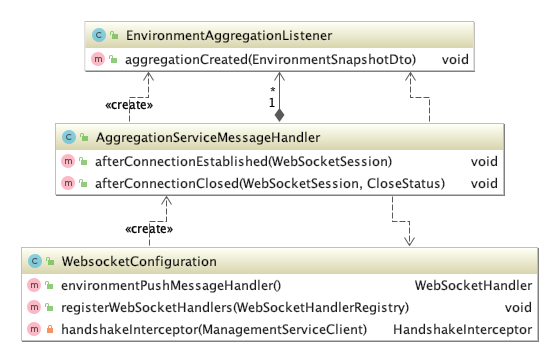
\includegraphics[width=\linewidth]{figures/impl/aggregation/websocket_package.png}
	\caption{Aggregation Service websocket package.}
	\label{aggregation_service_websocket_package}
\end{figure}

Aggregation domain objects are converted to equivalent Data Transfer Objects for dispatch to aggregation listeners. The information ultimately conveyed to listeners is described by Figure \ref{aggregation_service_dto_package}.

\begin{figure}[H]
	\centering  
	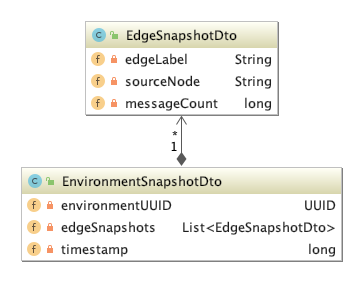
\includegraphics[scale=3.0]{figures/impl/aggregation/dto_package.png}
	\caption{Aggregation Service notification DTOs.}
	\label{aggregation_service_dto_package}
\end{figure}
 
\subsection{Aggregation Retention} \label{aggregation_service_message_retention}
The \texttt{Purge} module depicted in section \ref{aggregation_service_modules} is responsible for the flushing of persisted aggregations; the purge operation is performed at a configurable interval, with aggregations older than a configurable retention period being deleted from persistent storage. This functionality is intended to limit the application's use of disk space. 

\newpage
 
 \section{Correlation Service}
 
This microservice is responsible for the generation of correlation traces for messages observed in monitored environments, as described in section \ref{design_message_correlation}. An embedded web server hosting a GraphQL service provides a client interface for both users of the software and cooperating microservices. In this prototype implementation, the primary function of the Correlation Service is to support the Message Correlation Discovery Agent, discussed in section \ref{discovery_service_correlation_agent}. This microservice is implemented as a Spring Boot application.
 
 \subsection{Domain Model} \label{correlation_service_domain_model}
 The Correlation service domain model comprises three models. The Data Transfer Object pattern is used throughout this service. The first model, \texttt{CorrelationTraceDto}, models a single correlation trace for a monitored environment. It comprises a temporally ordered set of  \texttt{MessageDto} instances, each of which models a correlated message in a given monitored environment. Finally, an instance of  \texttt{CorrelationTraceFilterDto} is passed to the service by clients when requesting a correlation trace;  trace requests are specified by environment UUID and correlated field name. A class diagram is provided in Figure \ref{correlation_svc_domain_model}.
 
 \begin{figure}[H]
 	\centering  
 	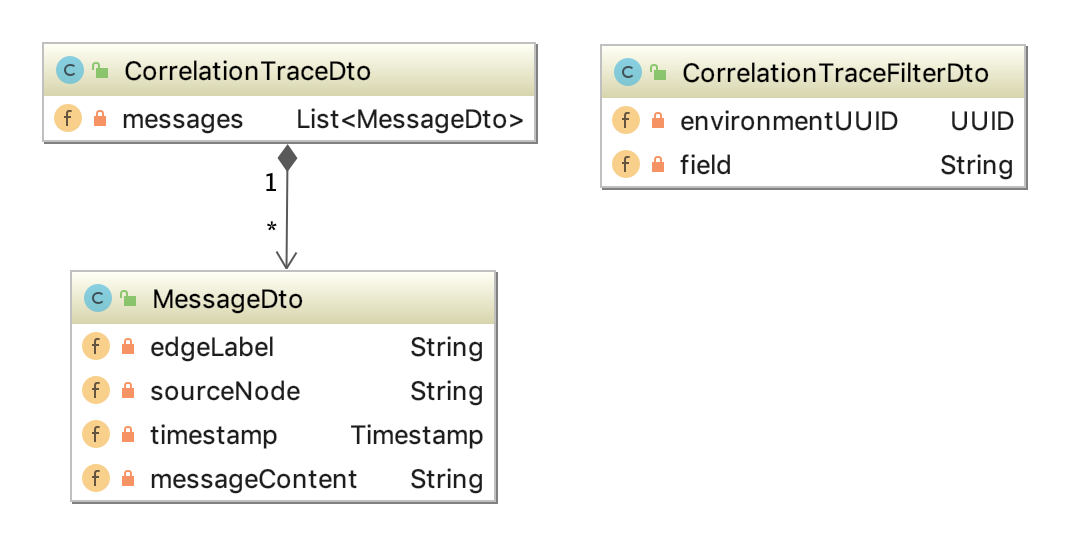
\includegraphics[scale=1.5] {figures/impl/correlation/domain.png}
 	\caption{Correlation Service domain model.}
 	\label{correlation_svc_domain_model}
 \end{figure}
  
 \subsection{Modules}
 The Correlation Service comprises the modules depicted in \ref{correlation_svc_modules}.  The structure is typical of a Spring Boot based microservice.
 
 \begin{figure}[H]
 	\centering  
 	\includegraphics[width=\linewidth]{figures/impl/correlation/modules.png}
 	\caption{Correlation Service modules.}
 	\label{correlation_svc_modules}
 \end{figure}

\subsection{Component Interactions}
The Correlation Service presents a single external interface. This interface provides a single query operation responsible for generation of correlation traces. A GraphQL \textit {CommandResolver} implements the external interface. It in turn invokes a \texttt{CorrelationService} interface, an implementation of which is responsible for trace generation, by querying the monitored message set via a  \texttt{DAO} module imported from the Monitoring Service. The simple sequence diagram presented in Figure  \ref{correlation_svc_seq_diagram} exemplifies the component interactions involved in generation of a correlation trace for a given environment.

\begin{figure}[H]
	\centering  
	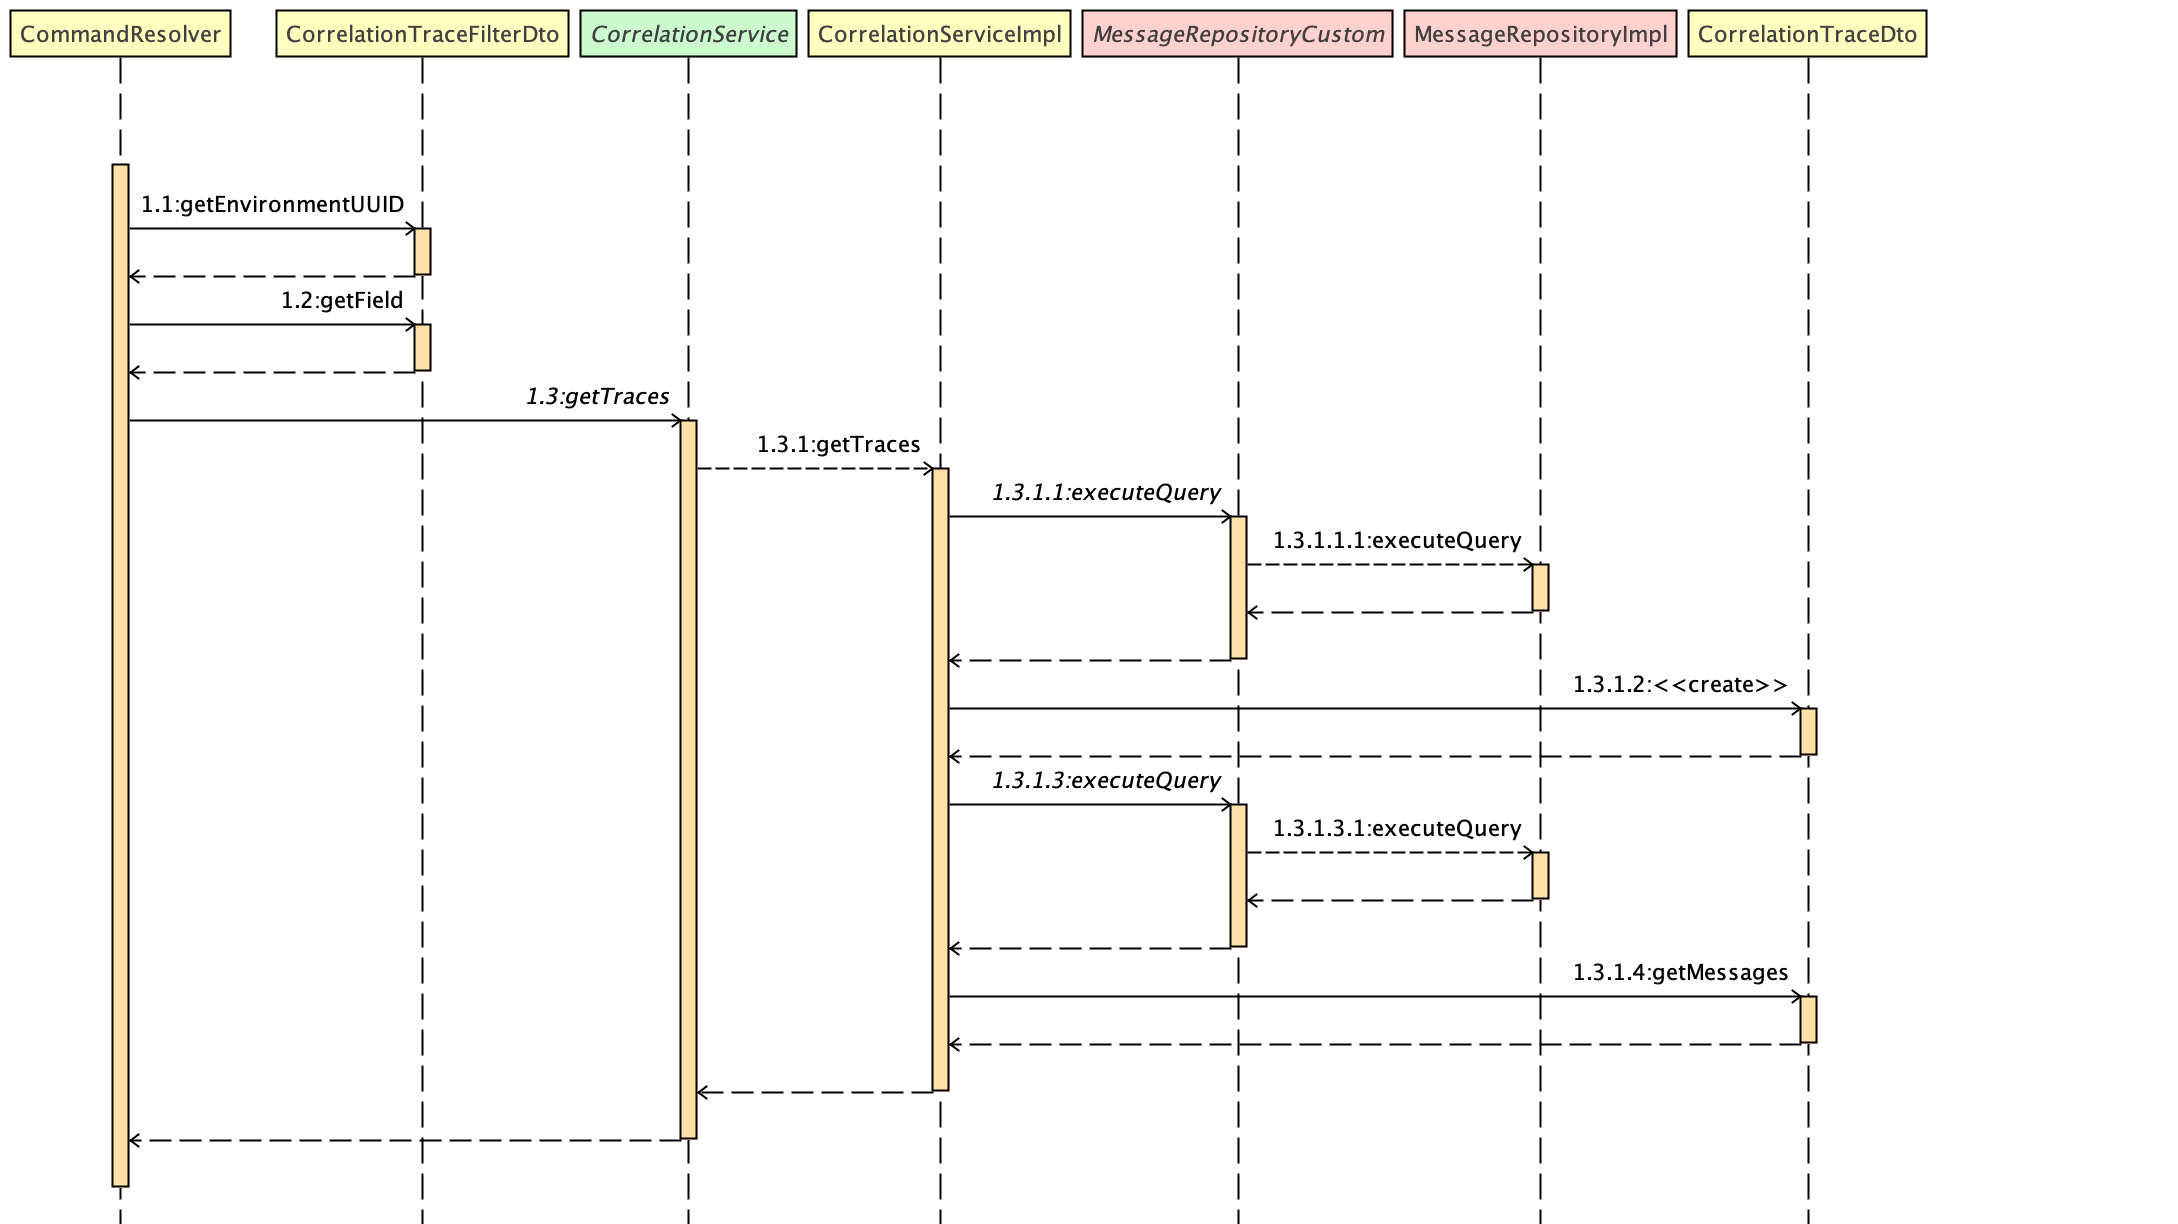
\includegraphics[width=\linewidth]{figures/impl/correlation/sequence.png}
	\caption{Sequence diagram: Requesting a correlation trace.}
	\label{correlation_svc_seq_diagram}
\end{figure}

\subsection{Correlation Algorithm}
A simple algorithm has been developed for message correlation. Correlation based on payload field value is facilitated by the Postgres-based monitored message repository, which supports JSON data types. Message payloads are persisted as JSON, allowing use of JSON-based search functions in message table queries. The Correlation Service leverages this feature when performing the following correlation steps:

\begin{itemize}
	\item Initialise an empty list \textit{L} of \texttt{CorrelationTraceDto} instances.
	\item Find all unique message field values monitored during the last hour.
	\item For each unique field value:
	\begin{itemize}
		\item Instantiate a \texttt{CorrelationTraceDto} instance \textit{CT} and add to \textit{L} .
		\item Determine the temporally-ordered set of messages whose payloads contain the unique field value.
		\item Construct a \texttt{MessageDto} for each message and add to \textit{CT}.
	\end{itemize}
\end{itemize}

 \newpage
 
 \section{Discovery Service}
 
This microservice is responsible for the discovery of environment topology information as discussed in section \ref{design_topology_discovery}, satisfying functional requirement \textit{FR-3}. It depends upon the Management Service for discovery of monitored environment information, synchronising periodically in order to start and stop sequentially executing topology discovery tasks. The implementation is agnostic of messaging technologies, in accordance with non-functional requirement \textit{NFR-2}.  A \textit{DiscoveryAgent API} provides for the implementation of varied discovery strategies, satisfying non-functional requirement \textit{NFR-1}. Two Discovery Agents, which are discussed in following sections, have been implemented as part of this prototype. Discovered topology information is registered with the Management Services via a client library exported by the latter. Discovered topology information is pushed to interested client such as the Dashboard Client using Spring WebSocket support.  This microservice is implemented as a Spring Boot application.
 
 \subsection{Modules}
 The Discovery Service comprises the modules depicted in \ref{discovery_svc_modules}. Modules which implement discovery agent plug-ins have been omitted from this diagram.
 
 \begin{figure}[H]
 	\centering  
 	\includegraphics[width=\linewidth]{figures/impl/discovery/modules.png}
 	\caption{Discovery Service modules.}
 	\label{discovery_svc_modules}
 \end{figure}

\subsection{Component Interactions}

The Discovery Service is driven by a scheduled discovery task which executes at a configurable interval, by default every five seconds. The discovery task first determines the set of currently monitored environments by polling the Management Service via its client module, as described in section \ref{management_service_external_interfaces}. The component interactions are depicted in Figure \ref{discovery_sync_task_sequence}.

\begin{figure}[H]
	\centering  
	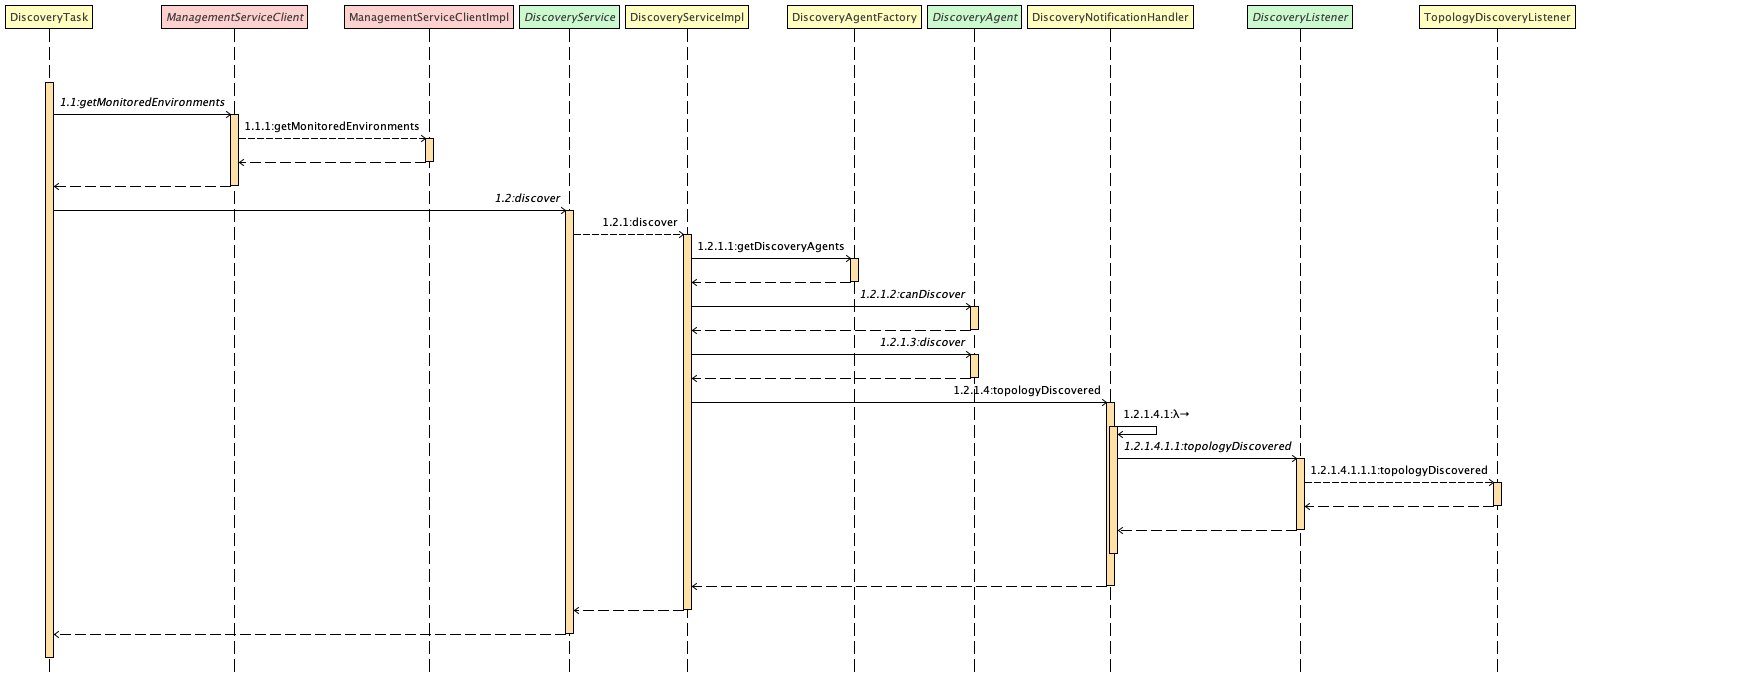
\includegraphics[width=\linewidth]{figures/impl/discovery/discovery_sequence.png}
	\caption{Discovery sequence diagram.}
	\label{discovery_sync_task_sequence}
\end{figure}

Having determined the set of currently monitored environments, the \texttt{DiscoveryTask} implementation passes these to the \texttt{DiscoveryService}, which in turns queries a \texttt{DiscoveryAgentFactory} to determine the set of available agents. For every monitored environment, the available agents are tested for applicability, and when found to be suitable candidates for environment discovery, are executed against a given environment. Discovery agent implementations are responsible for construction of \texttt{Topology} models, as described in section \ref{management_service_domain_model}. On discovery a Topology, a discovery event is dispatched to listeners registered with the \texttt{DiscoveryService}, as described in section \ref{discovery_service_notifications}.

\subsection{Discovery Agent API}
To extend the functionality of the software via addition of additional discovery strategies, the \texttt{Discovery} interface must be implemented, and the implementation class(es) made available on the runtime classpath of the Discovery Service. 

The developer of a \texttt{DiscoveryAgent} must define both Service Provider Interface (SPI) and API (Application Programming Interface) implementations. The \textit{Spring Factory} mechanism is leveraged to provide dynamic discovery and runtime auto-wiring of agent implementations \cite{SpringFactories}.

 The \texttt{DiscoveryAgent} \textit{discover()} method should construct and return an instance of \texttt{TopologyDto} to the calling application, which will in turn register the Topology with the Management Service. The Management Service will merge newly discovered Topology information with existing topology information for a given environment, preserving any existing topology structure.

This approach to topology discovery allows multiple discovery agents and strategies to construct an environment topology in a co-operative and incremental fashion if necessary.

When agent topology discovery is complete for a given scheduled execution of a \texttt{DiscoveryTask}, an asynchronous topology discovery event is dispatched to any registered listeners, as discussed in section \ref{discovery_service_notifications}.

\begin{figure}[H]
	\centering  
	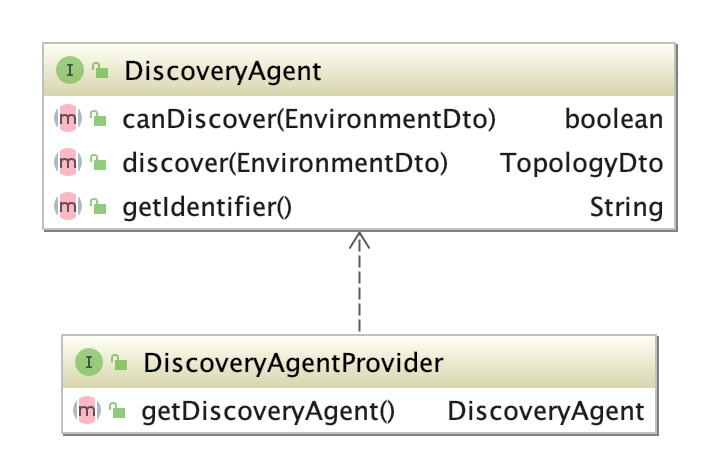
\includegraphics[scale=2.0]{figures/impl/discovery/agent_api.png}
	\caption{DiscoveryAgent SPI and API.}
	\label{discovery_agent_api}
\end{figure}

\subsection{Discovery Notifications} \label{discovery_service_notifications}
The Discovery Service implements a single external interface, closely resembling that implemented by the Aggregation Service, as described in section \ref{aggregation_service_notifications}. Clients may register for environment-specific Topology update events via a WebSocket interface.

Instances of \texttt{TopologyDto} are serialized to JSON and pushed to registered client listeners. The TopologyDto type is described by Figure \ref{topology_dto}.

\begin{figure}[H]
	\centering  
	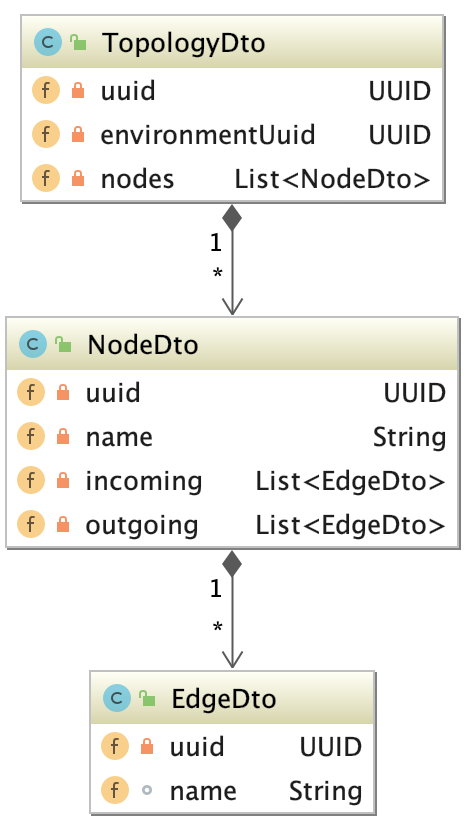
\includegraphics[scale=1.5]{figures/impl/discovery/topology_dto.png}
	\caption{Topology DTO.}
	\label{topology_dto}
\end{figure}

\subsection{Discovery Agent Implementation - Kubernetes Discovery Agent} 

The design of this agent implementation is discussed in Section \ref{design_kubernetes_discovery_agent}. The agent determines whether it can perform discovery for a given environment based on the following criteria:

\begin{itemize}
	\item The environment must define the following configuration properties:
	\begin{itemize}
	\item \texttt{discovery.agent.k8s.cert.path}: the filesystem path at which a certificate for the target Kubernetes environment can be found.
	\item \texttt{discovery.agent.k8s.namespace}:The Kubernetes namespace in which configmaps for the target environment can be discovered.
	\end{itemize}
\end{itemize}

As this agent consumes technology-agnostic metadata from Kubernetes configmaps, it is usable with various messaging technologies.

The agent is enabled by simply adding it to the classpath of the Discovery Service, as demonstrated by the following Maven POM snippet:

\begin{lstlisting}
<dependency>
  <groupId>org.cit.mcaleerj.thesis.discovery</groupId>
  <artifactId>k8s-discovery-agent</artifactId>
  <version>0.0.1-SNAPSHOT</version>
</dependency>
\end{lstlisting}

\subsection{Discovery Agent Implementation - Message Correlation}\label{discovery_service_correlation_agent} 

The design of this agent implementation is discussed in Section \ref{design_message_correlation}. The agent determines whether it can perform discovery for a given environment based on the following criteria:

\begin{itemize}
	\item The environment must define the following configuration property:
	\begin{itemize}
		\item \texttt{discovery.agent.correlation.field.name}: the message payload field used to correlate messages and construct correlation traces.
	\end{itemize}
\end{itemize}

As this agent performs correlation on technology-agnostic messages persisted by the Monitoring Service, it is usable with various messaging technologies.

The agent is enabled by simply adding it to the classpath of the Discovery Service, as demonstrated by the following Maven POM snippet:

 \vspace{5mm}
 
\begin{lstlisting}
<dependency>
<groupId>org.cit.mcaleerj.thesis.discovery</groupId>
<artifactId>message-correlation-discovery-agent</artifactId>
<version>0.0.1-SNAPSHOT</version>
</dependency>
\end{lstlisting}

 \newpage
 
 \section{User Interface Service}
 
 The User Interface service is a simple Spring Boot microservice which serves static resources required by the client dashboard application.  
 
 \section{Dashboard Client}
 
 The design of this component is discussed in section \ref{design_client_dashboard}. The Dashboard has been implemented as a Dagre-D3 based, single-page web application, served to clients by the User Interface Service. Users of the dashboard load the application by pointing a browser at the application URL, which must contain the monitored environment UUID as retrieved from the Management Service GraphQL interface. On loading, the Dashboard performs the following steps:
 
\begin{enumerate}
\item Determine the environment UUID for which the Dashboard has been opened.
\item Open a WebSocket connection to the Discovery Service, via the Gateway Service, subscribing to notifications for the given environment UUID. 
\item Open a WebSocket connection to the Aggregation Service, via the Gateway Service, subscribing to notifications for the given environment UUID. 
\item On receipt of an asynchronous event from the Discovery Service:
	\begin{enumerate}
		\item Construct a topology model by deserialising the discovery event payload.
		\item Generate a topology hash. Compare the hash value to the last rendered topology hash; ignore the discovery event if hash codes match.
		\item If topology has not already been rendered, transform the received topology object to the graph format expected by the Dagre-D3 client library, then render the graph. Furthermore, render the monitored environment name to the browser page.
	\end{enumerate}
\item On receipt of an asynchronous event from the Aggregation Service:
\begin{enumerate}
	\item Construct an EnvironmentAggregation model (see section \ref{aggregation_service_domain_model}) by deserialising the aggregation event payload.
	\item Render the aggregation window details to the browser page.
	\item For each Edge Aggregation contained in the Aggregation model, locate the corresponding graph edge, then render activity information to same.
\end{enumerate}
\end{enumerate}

The graph styling discussed in section \ref{design_topology_visualisation} has been achieved by leveraging APIs provided by the Dagre-D3 library. Results are demonstrated in Chapter 6. 

 \section{Service Registry}
 
 The Service Registry implements a simple Eureka-based discovery server. Eureka, developed by Netflix, is a REST based service which allows microservices to locate and communicate with each other without the need for hard-coding host and port details in the various co-operating service instances. The following services are configured as Eureka clients:
 
 \begin{itemize}
 	\item Management Service
 	\item Monitoring Service
 	\item Aggregation Service
 	\item Discovery Service
 	\item Correlation Service
	\item User Interface Service
	\item Gateway Service
 \end{itemize}

On startup, each service registers itself with the Service Registry, using a unique service identifier. Thereafter, lookups for the service instance endpoint information are performed via the registry. This mechanism is depicted in Figure \ref{service_registry_scheme}.
 
\begin{figure}[H]
	\centering  
	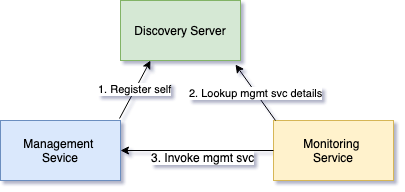
\includegraphics[scale=0.8]{figures/impl/registry/eureka_discovery.png}
	\caption{Service discovery via Service Registry.}
	\label{service_registry_scheme}
\end{figure}

\newpage

 \section{Gateway Service}
 
 The Gateway service is a Spring Boot microservice based on the Spring Cloud Gateway project. The gateway presents a single point of access for clients of the monitoring application, by routing incoming requests to downstream services, while simultaneously functioning as a proxy for asynchronous WebSocket messages. 
 
 \vspace{5mm}
 
 \begin{figure}[H]
 	\centering  
 	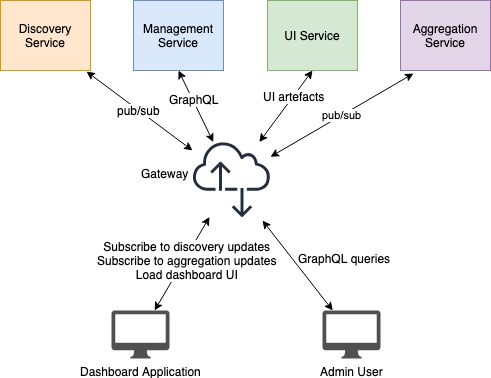
\includegraphics[scale=0.8]{figures/impl/gateway/gateway.png}
 	\caption{Gateway Service routing.}
 	\label{gatway_service}
 \end{figure}

 The following routes are implemented by the Gateway Service:
 
  \begin{itemize}
 	\item HTTP requests to load the monitoring dashboard UI are routed to the UI service.
 	\item WebSocket connections are routed to the Discovery and Aggregation services.
 	\item GraphQL requests are routed to the Management Service.
 \end{itemize}

The Gateway Service integrates with the Discovery Service, resolving route destinations via the latter service.
 
 \newpage
 
 \section{Kafka Message Producer Identification}\label{software_impl_producer_ident} 
 
 The strategy described in Section \ref{kafka_producer_header_design} has been used to develop a Spring library which enables transparent addition of message producer identifier information to Kafka messages produced by Spring applications. The library is named \textbf{spring-kafka-producer-headers}.
 
 The library comprises a single configuration class which is loaded by the Spring framework during initialisation by means of the Spring auto-configuration mechanism \cite{SpringFactories}. The configuration class returns a \texttt{BeanPostProcessor} instance to the framework; thereafter, all beans instantiated by the framework are inspected by this post-processor. The steps implemented by the post-processor are as follows:
 
 \begin{itemize}
  	\item Determine whether the passed bean is of interest - does it represent a message channel?
  	\item If so, determine whether the message channel is an output channel.
  	\item If so, add an interceptor to the channel. 
  	\item The channel interceptor will add a message header identifying the sending application to every produced message.
 \end{itemize}

To enable automatic addition of Kafka producer headers to a Spring application, a dependency on this library is simply added to the application's dependency set. No other changes are required.

For an application that uses Maven for dependency management, addition of the following dependency will enable production of Kafka headers:

\vspace{5mm}

\begin{lstlisting}[caption={Maven dependency on spring-kafka-producer-headers},captionpos=b]
<dependencies>
  <dependency>
    <groupId>org.cit.mcaleerj.thesis.spring-kafka</groupId>
    <artifactId>spring-kafka-producer-headers</artifactId>  
  </dependency>
</dependencies>
\end{lstlisting}


 